\documentclass{standalone}

\usepackage{tikz}
\usepackage{tkz-euclide}
\usetikzlibrary{calc}
\usetikzlibrary{positioning}
\usetikzlibrary{arrows.meta}

\usepackage{times}


\begin{document}
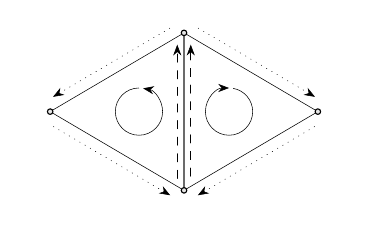
\begin{tikzpicture}[%
  >={Stealth[scale=1.0]},
]

  \tkzDefPoint(0.0, 0.0){A}
  \tkzDefPoint(1.7, -1.0){B}
  \tkzDefPoint(1.7, 1.0){C}
  \tkzDefPoint(3.4, 0.0){D}

  \tkzInCenter(A,B,C)\tkzGetPoint{C1}
  \tkzDefPointOnCircle[R = center C1 angle 90 radius 0.3]\tkzGetPoint{U}
  \tkzDefPointOnCircle[R = center C1 angle 80 radius 0.3]\tkzGetPoint{V}
  \tkzDrawArc[color=black,->](C1,U)(V)

  \tkzInCenter(B,C,D)\tkzGetPoint{C2}
  \tkzDefPointOnCircle[R = center C2 angle 90 radius 0.3]\tkzGetPoint{U}
  \tkzDefPointOnCircle[R = center C2 angle 80 radius 0.3]\tkzGetPoint{V}
  \tkzDrawArc[color=black,<-](C2,U)(V)

  \tkzDrawPolygon(A,B,C)
  \tkzDrawPolygon(B,C,D)

  \tkzDefPointOnLine[pos=0.85](C1,B)\tkzGetPoint{L1}
  \tkzDefPointOnLine[pos=0.85](C1,C)\tkzGetPoint{L2}
  \tkzDrawSegment[dashed,->](L1,L2)

  \tkzDefPointOnLine[pos=1.25](C1,B)\tkzGetPoint{LB1}
  \tkzDefPointOnLine[pos=1.25](C1,A)\tkzGetPoint{LB2}
  \tkzDrawSegment[add=-0.15 and -0.15,dotted,<-](LB1,LB2)
  \tkzDefPointOnLine[pos=1.25](C1,A)\tkzGetPoint{LT1}
  \tkzDefPointOnLine[pos=1.25](C1,C)\tkzGetPoint{LT2}
  \tkzDrawSegment[add=-0.15 and -0.15,dotted,<-](LT1,LT2)

  \tkzDefPointOnLine[pos=0.85](C2,B)\tkzGetPoint{R1}
  \tkzDefPointOnLine[pos=0.85](C2,C)\tkzGetPoint{R2}
  \tkzDrawSegment[dashed,<-](R2,R1)

  \tkzDefPointOnLine[pos=1.25](C2,B)\tkzGetPoint{RB1}
  \tkzDefPointOnLine[pos=1.25](C2,D)\tkzGetPoint{RB2}
  \tkzDrawSegment[add=-0.15 and -0.15,dotted,<-](RB1,RB2)
  \tkzDefPointOnLine[pos=1.25](C2,D)\tkzGetPoint{RT1}
  \tkzDefPointOnLine[pos=1.25](C2,C)\tkzGetPoint{RT2}
  \tkzDrawSegment[add=-0.15 and -0.15,dotted,<-](RT1,RT2)

  \tkzDrawPoints(A,B,C,D)

\end{tikzpicture}
\end{document}
